\chapter{Airframe \& Supporting Systems}
\label{ch:airframe}

% \section{\ac{uas} Operational Approval}\label{sec:uasapproval}

% \section{Configuration Management and Documentation}\label{sec:uasconfiguration}

\section{System Specifications}\label{sec:systemspecs}
    \subsection{Frame Design}
        The MARS unmanned aircraft system (UAS) utilizes an X-shaped quadrotor frame configuration with four propellers. This design optimizes thrust-to-weight ratio while maintaining structural simplicity and ease of construction.
        
        The primary frame structure is constructed from garolite (G10 fiberglass), providing high strength, thermal resistance, and electrical insulation. The aircraft arms are 15.5-inch members fabricated from 16 mm outer diameter carbon fiber tubing, selected to accommodate T-Motor P17x5.8 propellers and provide sufficient rigidity under load.
        
    \subsection{Critical Hardware Components}
    \subsubsection{} Critical hardware components are sourced from non-adversarial vendors to ensure compliance with NDAA and Blue UAS requirements.
    
    \subsubsection{Flight Controller} The system is centered around a Cube Orange+ flight controller, which provides onboard processing and integrates multiple sensors, including inertial measurement units (IMUs) and barometers, enabling stable and autonomous flight operations.
    
    \subsubsection{GPS} Navigation is supported by a CubePilot Here4 GNSS module, which serves as the primary GPS onboard the MARS aircraft.
    
    \subsubsection{Rangefinder} Obstacle detection capability is provided by a LightWare LW20/C laser rangefinder, which delivers precise distance measurements for enhanced situational awareness during flight.
    
    \subsubsection{Motors} The propulsion system consists of four KDE 3520XF brushless motors, each supporting propellers up to 18.5 inches and operating within a voltage range of 14.8 V to 34.8 V (4S–8S LiPo). These motors are paired with KDE UAS35 electronic speed controllers (ESCs), which support up to 35 A continuous current and operate within a voltage range of 7.4 V to 34.8 V.
    
    \subsubsection{Battery} Power is supplied by a Tattu 23,000 mAh 6C LiPo battery and distributed via an FCHUB-12S V2 power distribution board (PDB). The PDB provides regulated 5 V output for the flight controller and onboard communication systems.
    
    \subsubsection{ADS-B} To enhance airspace awareness and comply with FAA requirements, the aircraft is equipped with an ADS-B receiver for detection of nearby cooperative aircraft.

    \begin{figure}
        \centering
        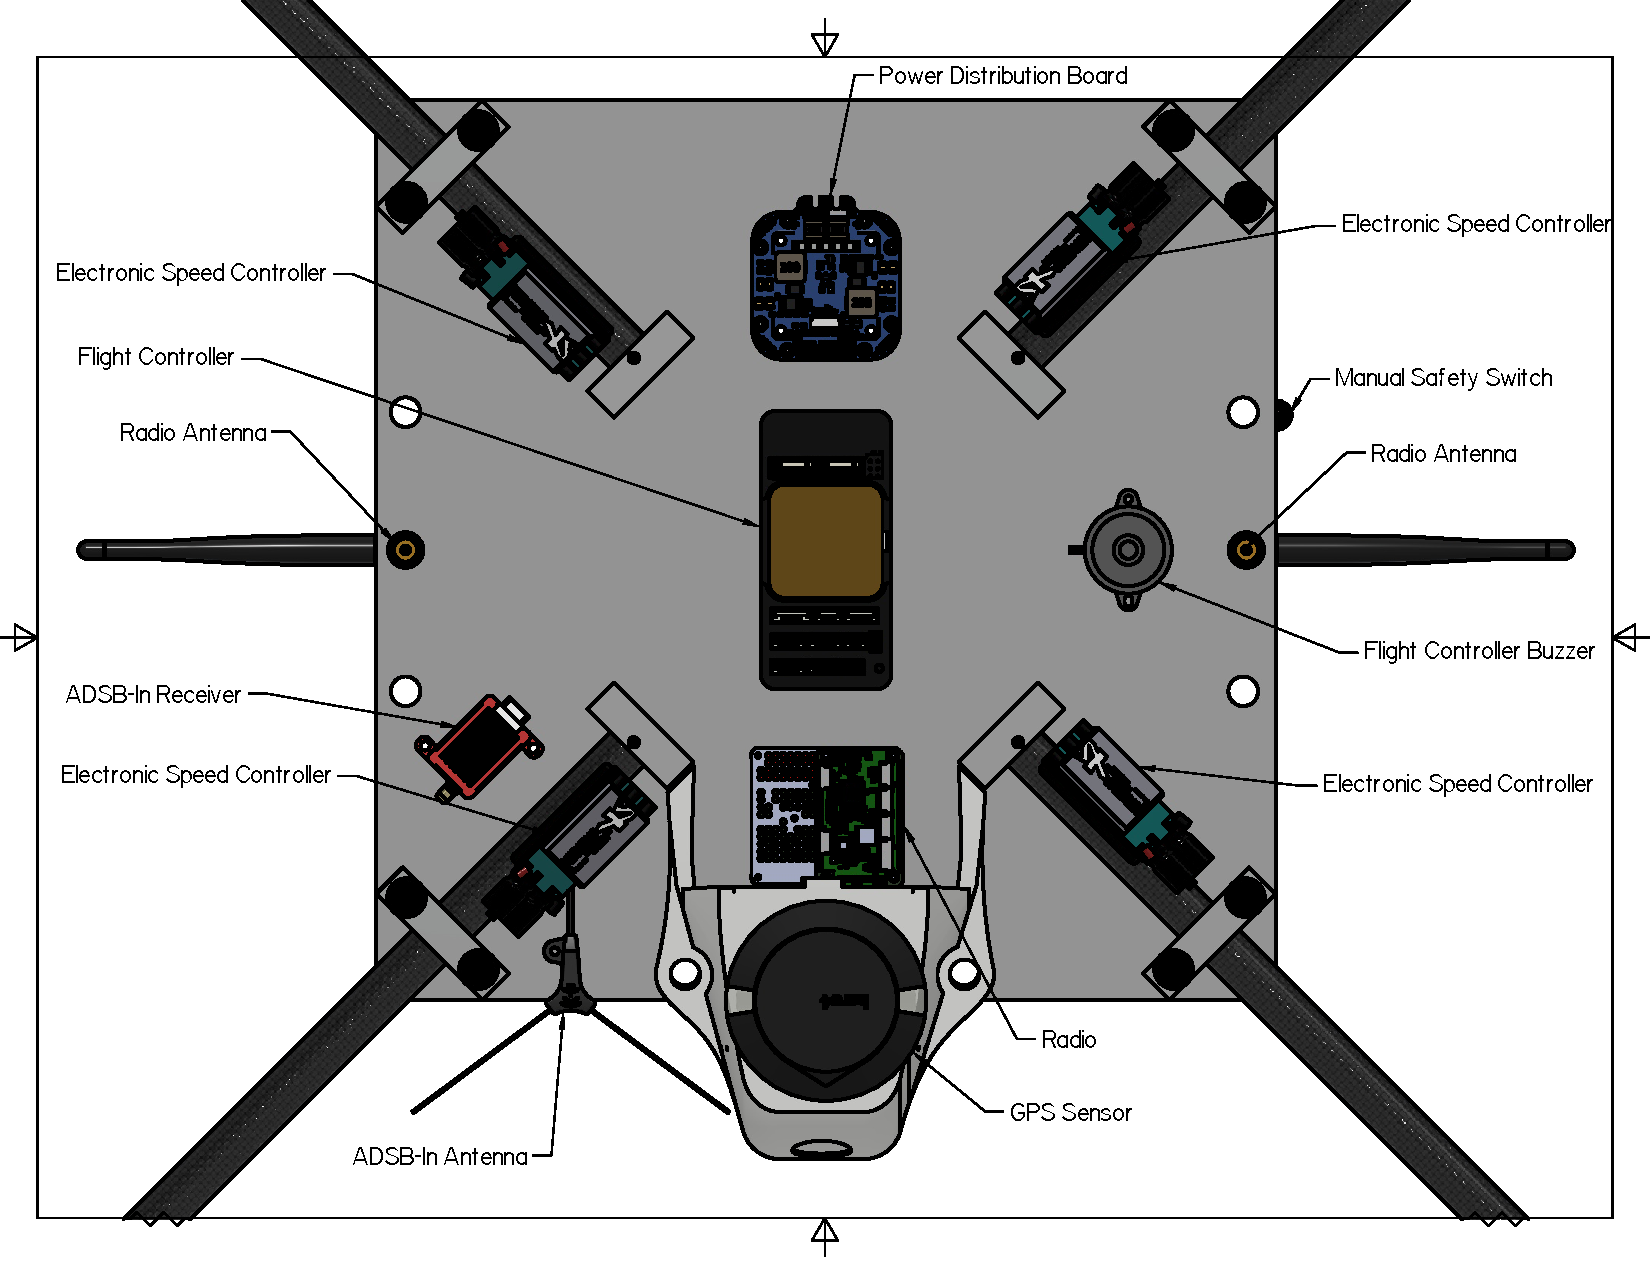
\includegraphics[width=1\textwidth]{system_diagrams/system_diagrams_Part1.pdf}
        \caption{Overhead View of Critical Components}
        \label{fig:SystemDiagram1}
    \end{figure}

    \begin{figure}
        \centering
        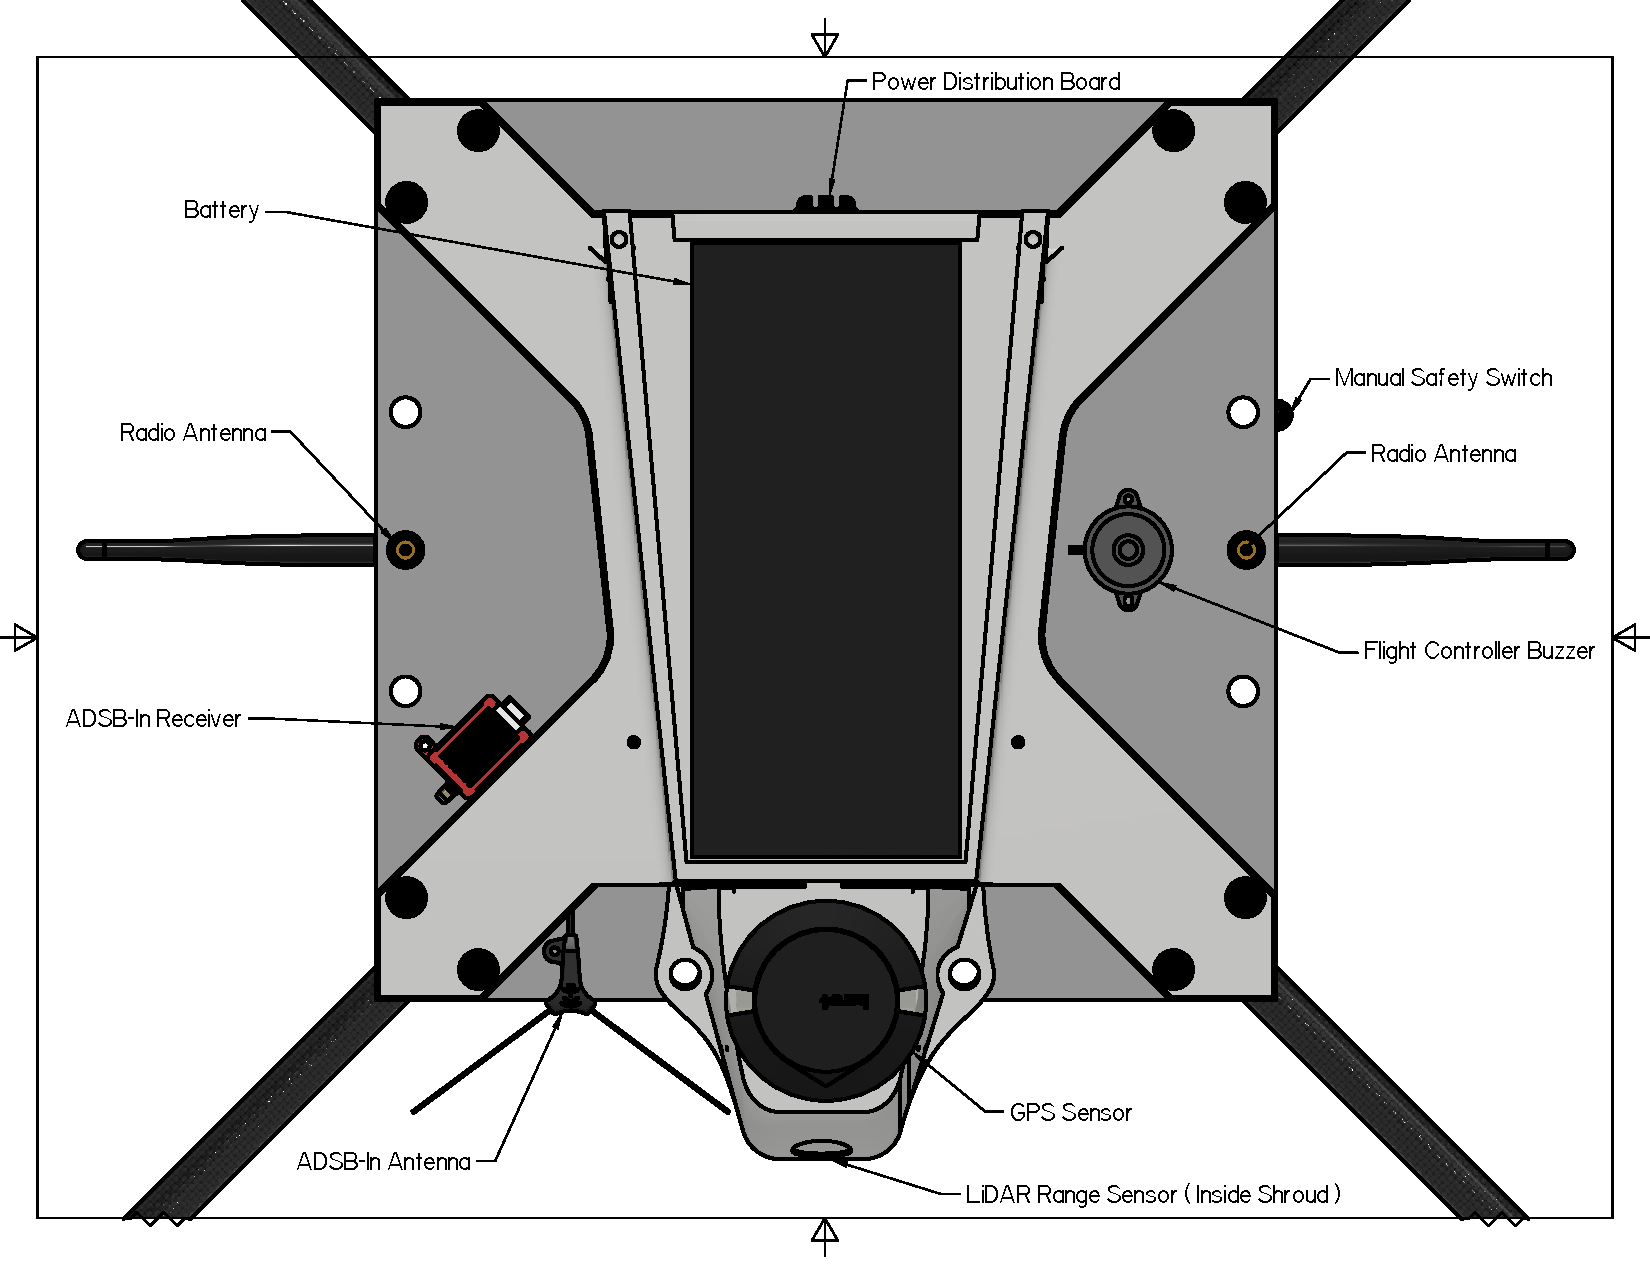
\includegraphics[width=1\linewidth]{system_diagrams/system_diagrams_Part2.pdf}
        \caption{Overhead View with Battery Shroud}
        \label{fig:SystemDiagram2}
    \end{figure}

    \begin{figure}
        \centering
        \makebox[\textwidth][c]{%
            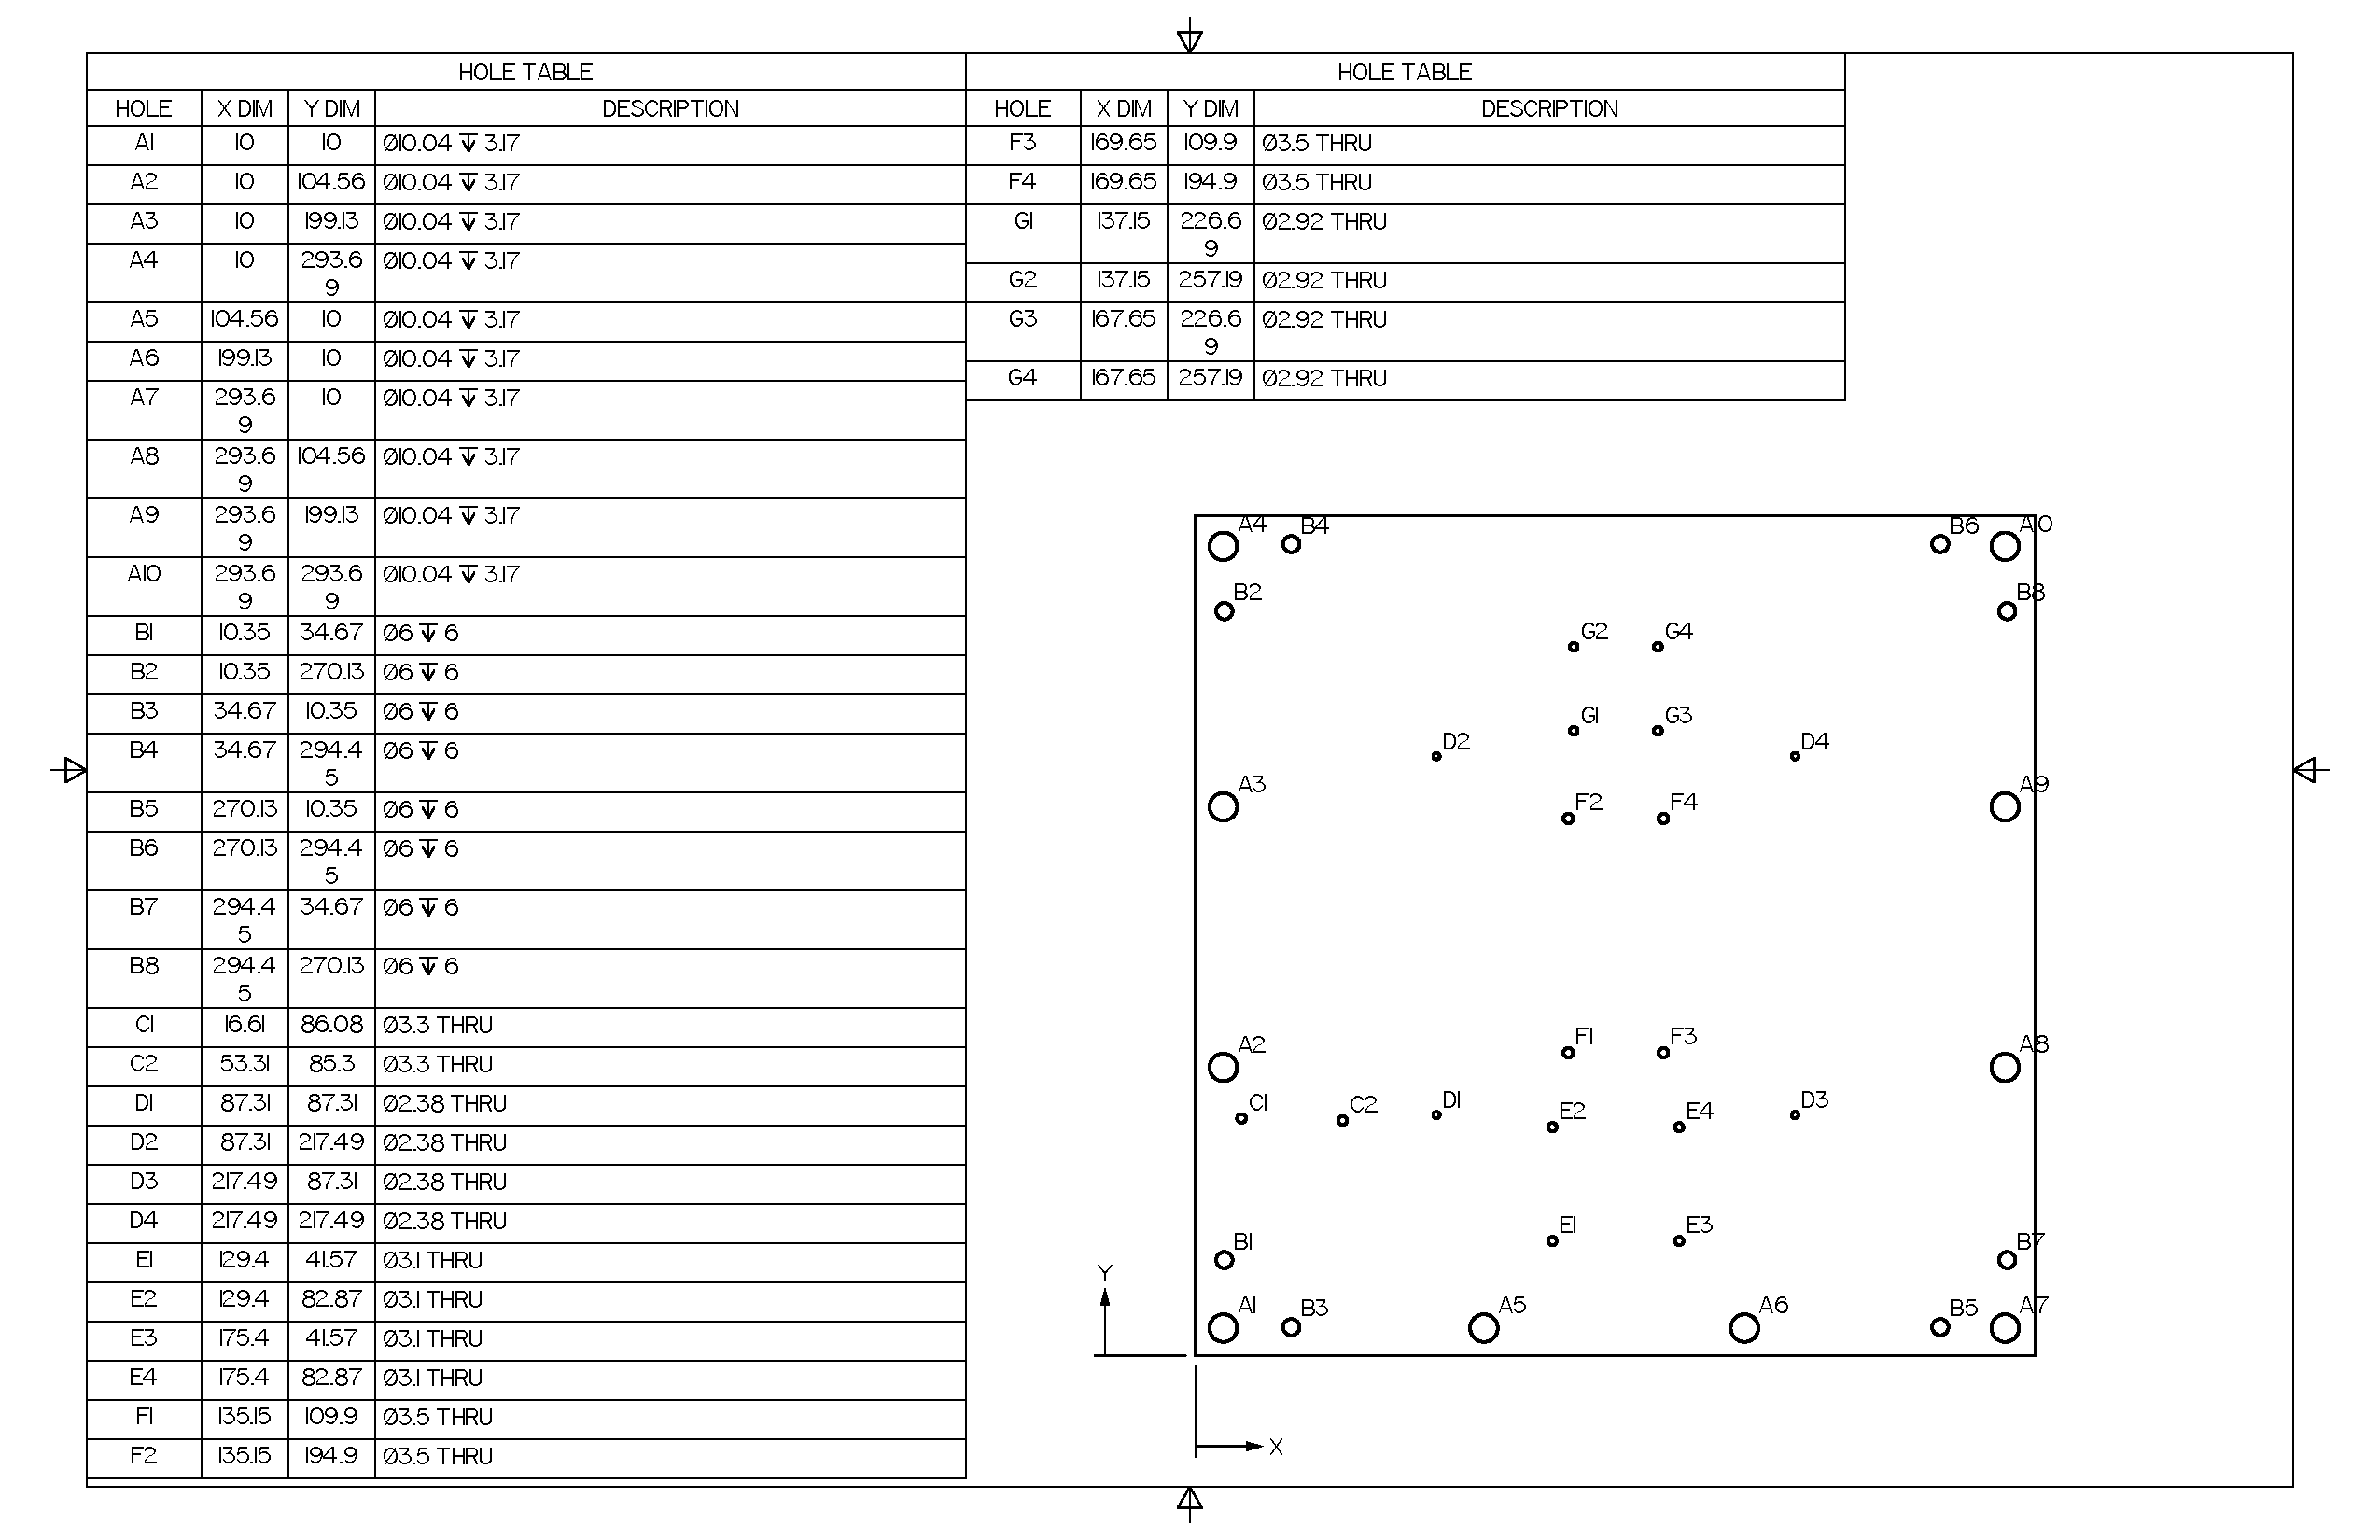
\includegraphics[width=0.9\paperwidth]{system_diagrams/system_diagrams_Part3.pdf}
        }
        \caption{Middle Plate Screw Hole Dimensions (All Measurements in Millimeters)}
        \label{fig:SystemDiagram3}
    \end{figure}

    \begin{figure}
        \centering
        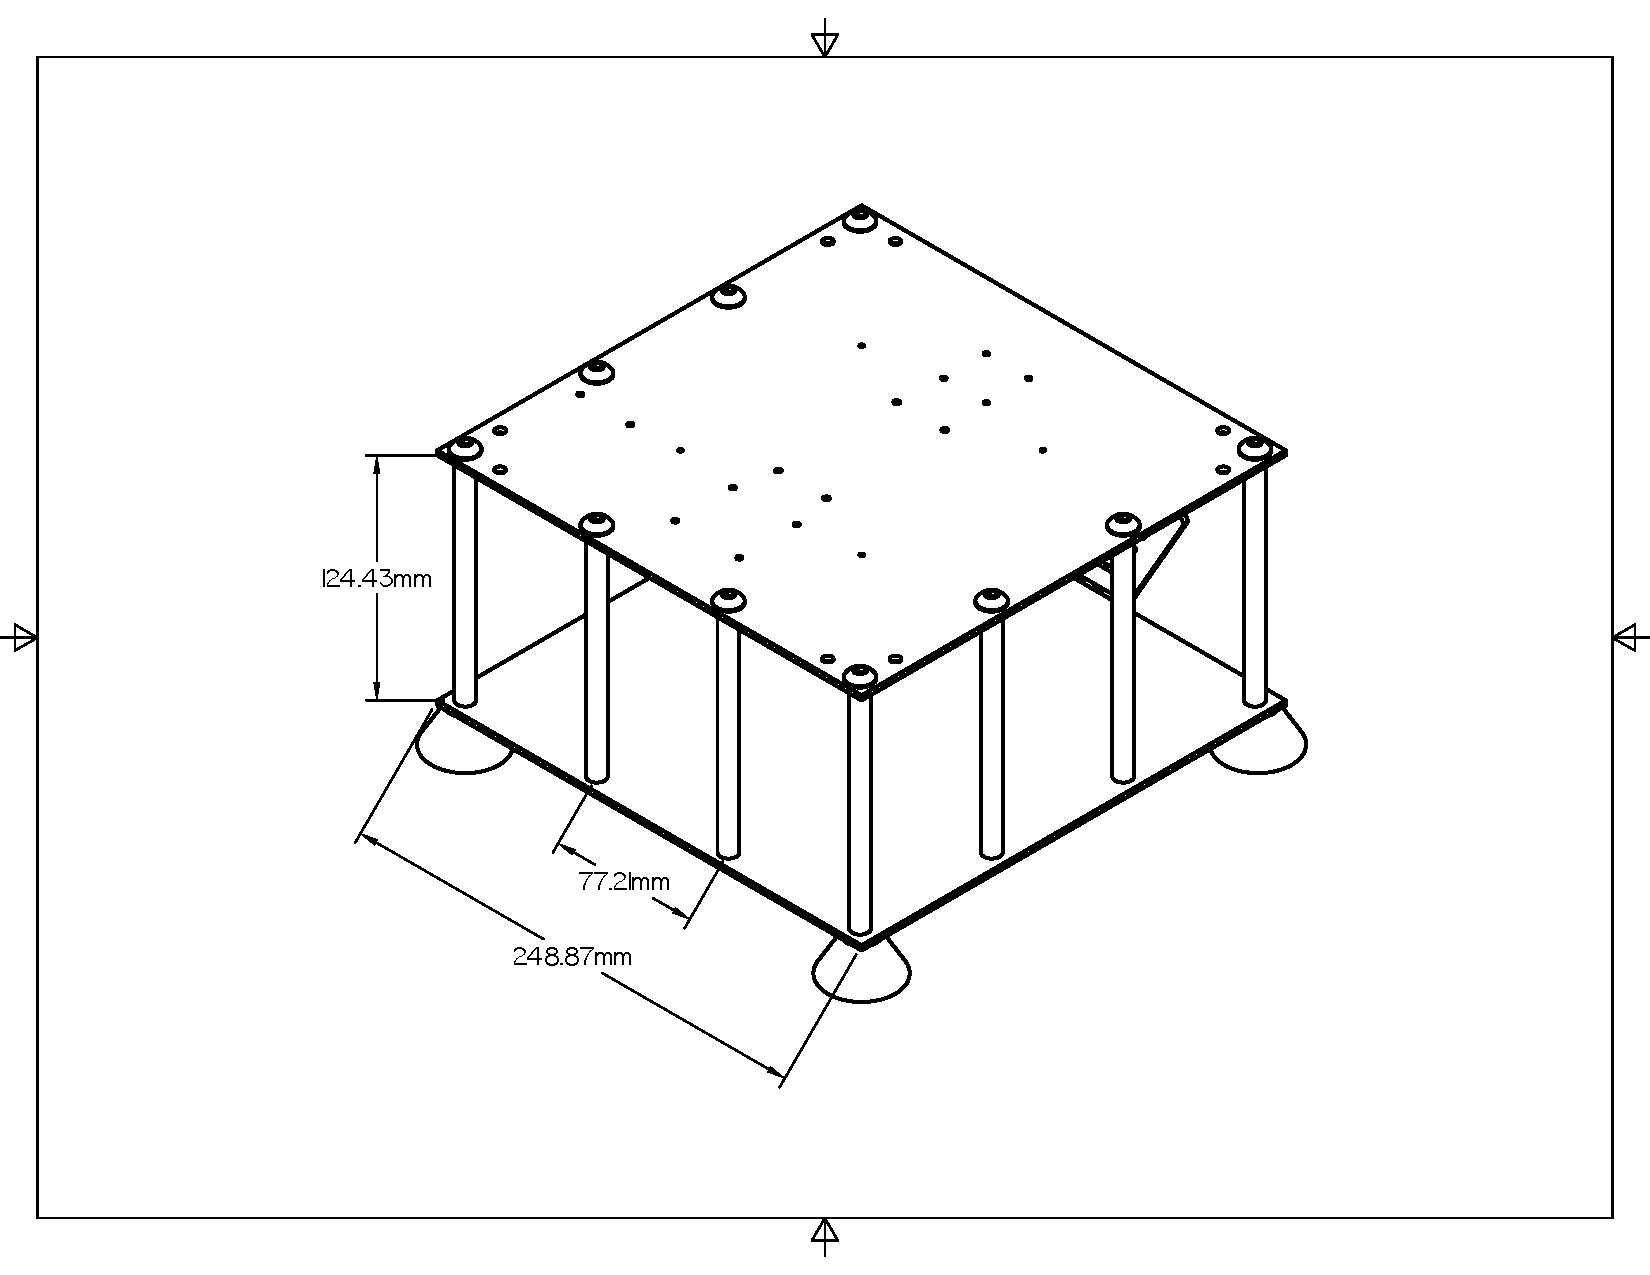
\includegraphics[width=1\linewidth]{system_diagrams/system_diagrams_Part4.pdf}
        \caption{Isometric View of Cargo Bay}
        \label{fig:SystemDiagram4}
    \end{figure}

    \begin{figure}
        \centering
        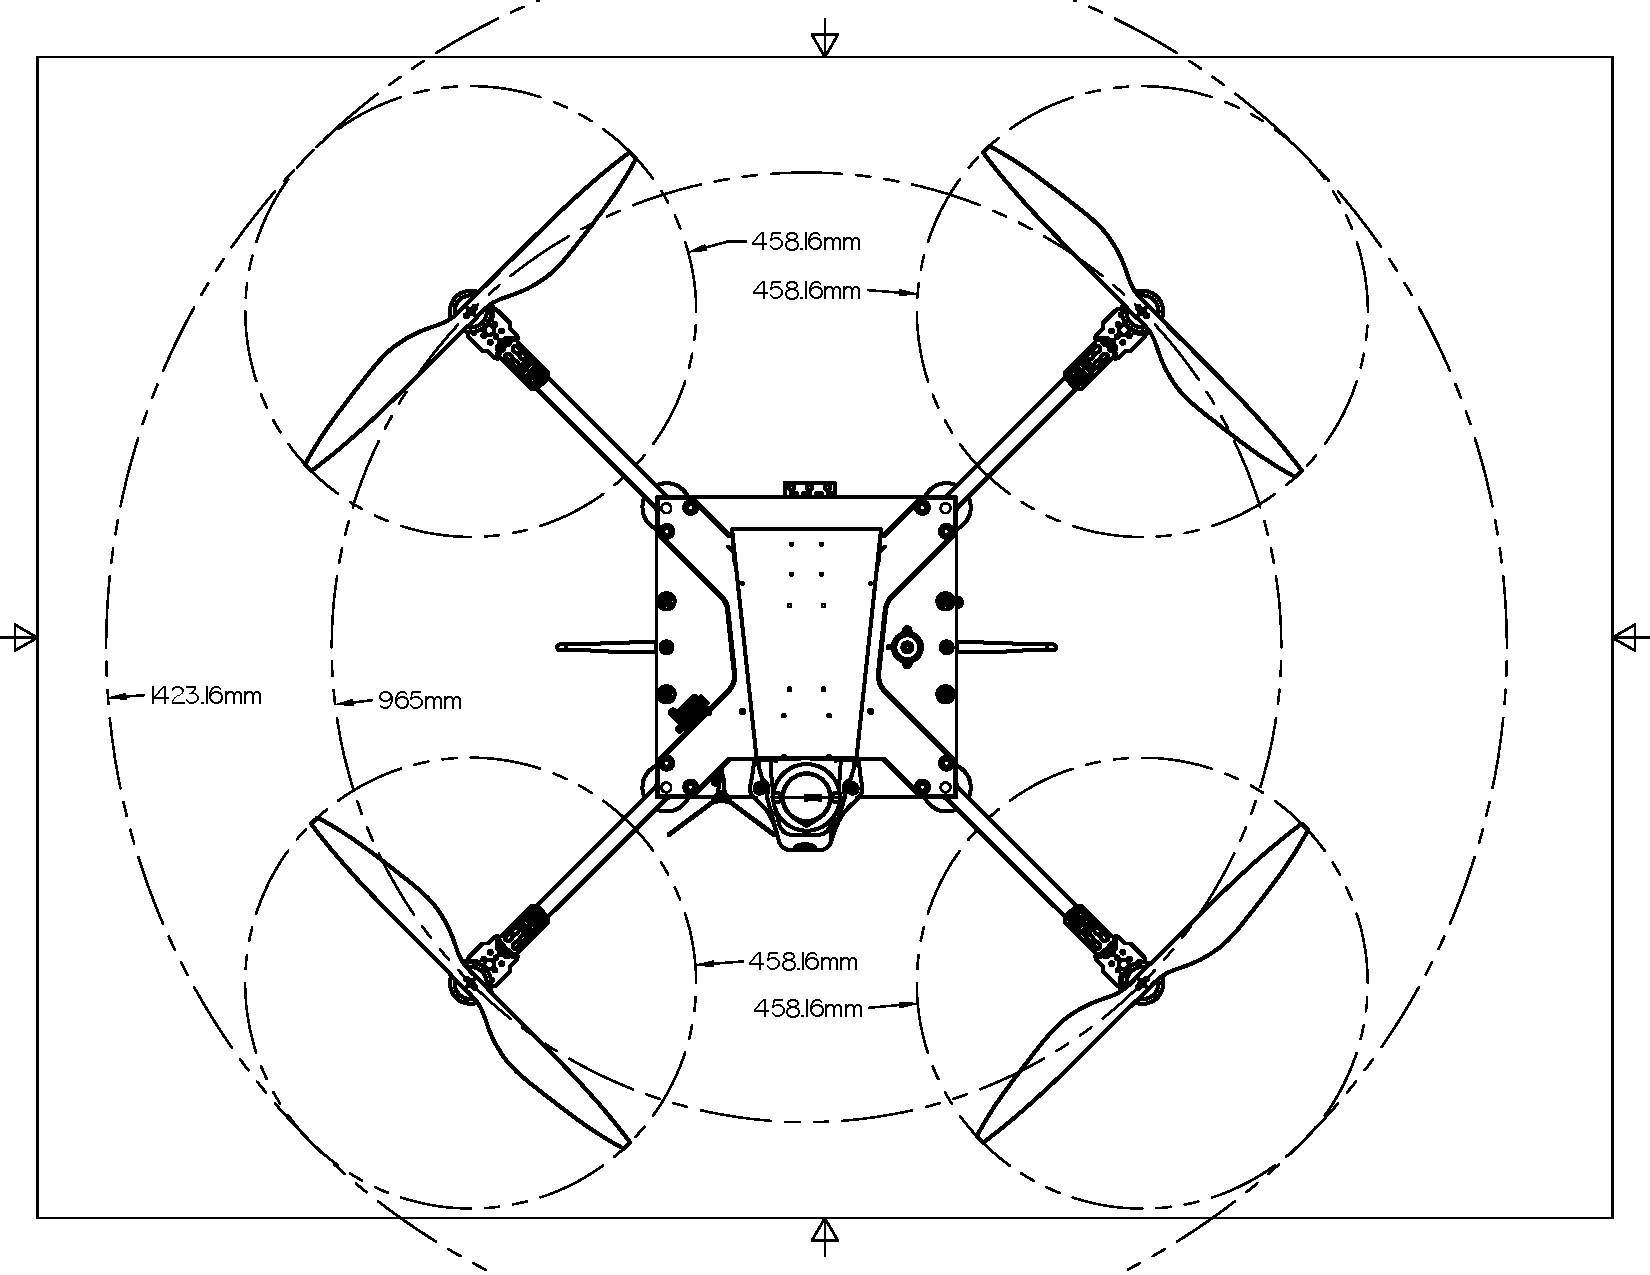
\includegraphics[width=1\linewidth]{system_diagrams/system_diagrams_Part5.pdf}
        \caption{Propeller Distances and Diameters}
        \label{fig:SystemDiagram5}
    \end{figure}

    \begin{figure}
        \centering
        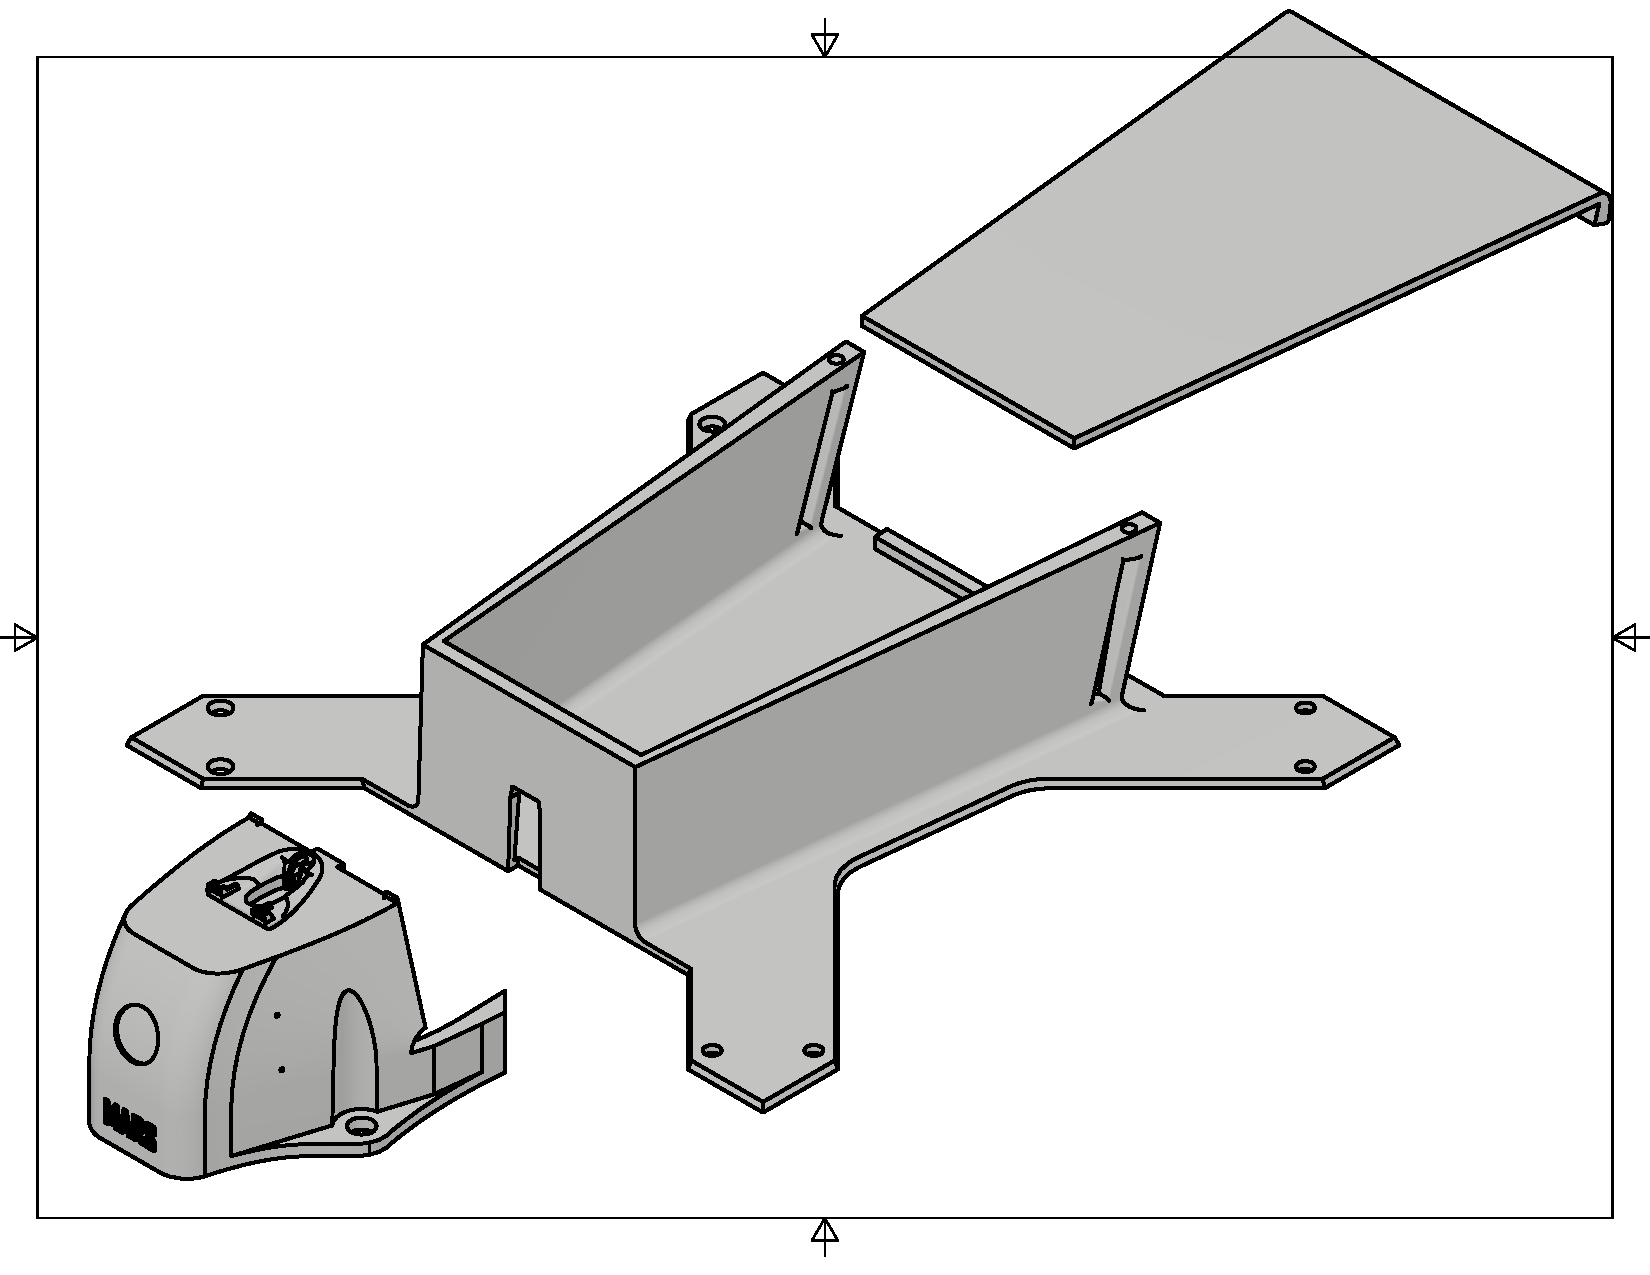
\includegraphics[width=1\linewidth]{system_diagrams/system_diagrams_Part6.pdf}
        \caption{Battery Shroud Composition}
        \label{fig:SystemDiagram6}
    \end{figure}

    \begin{figure}
        \centering
        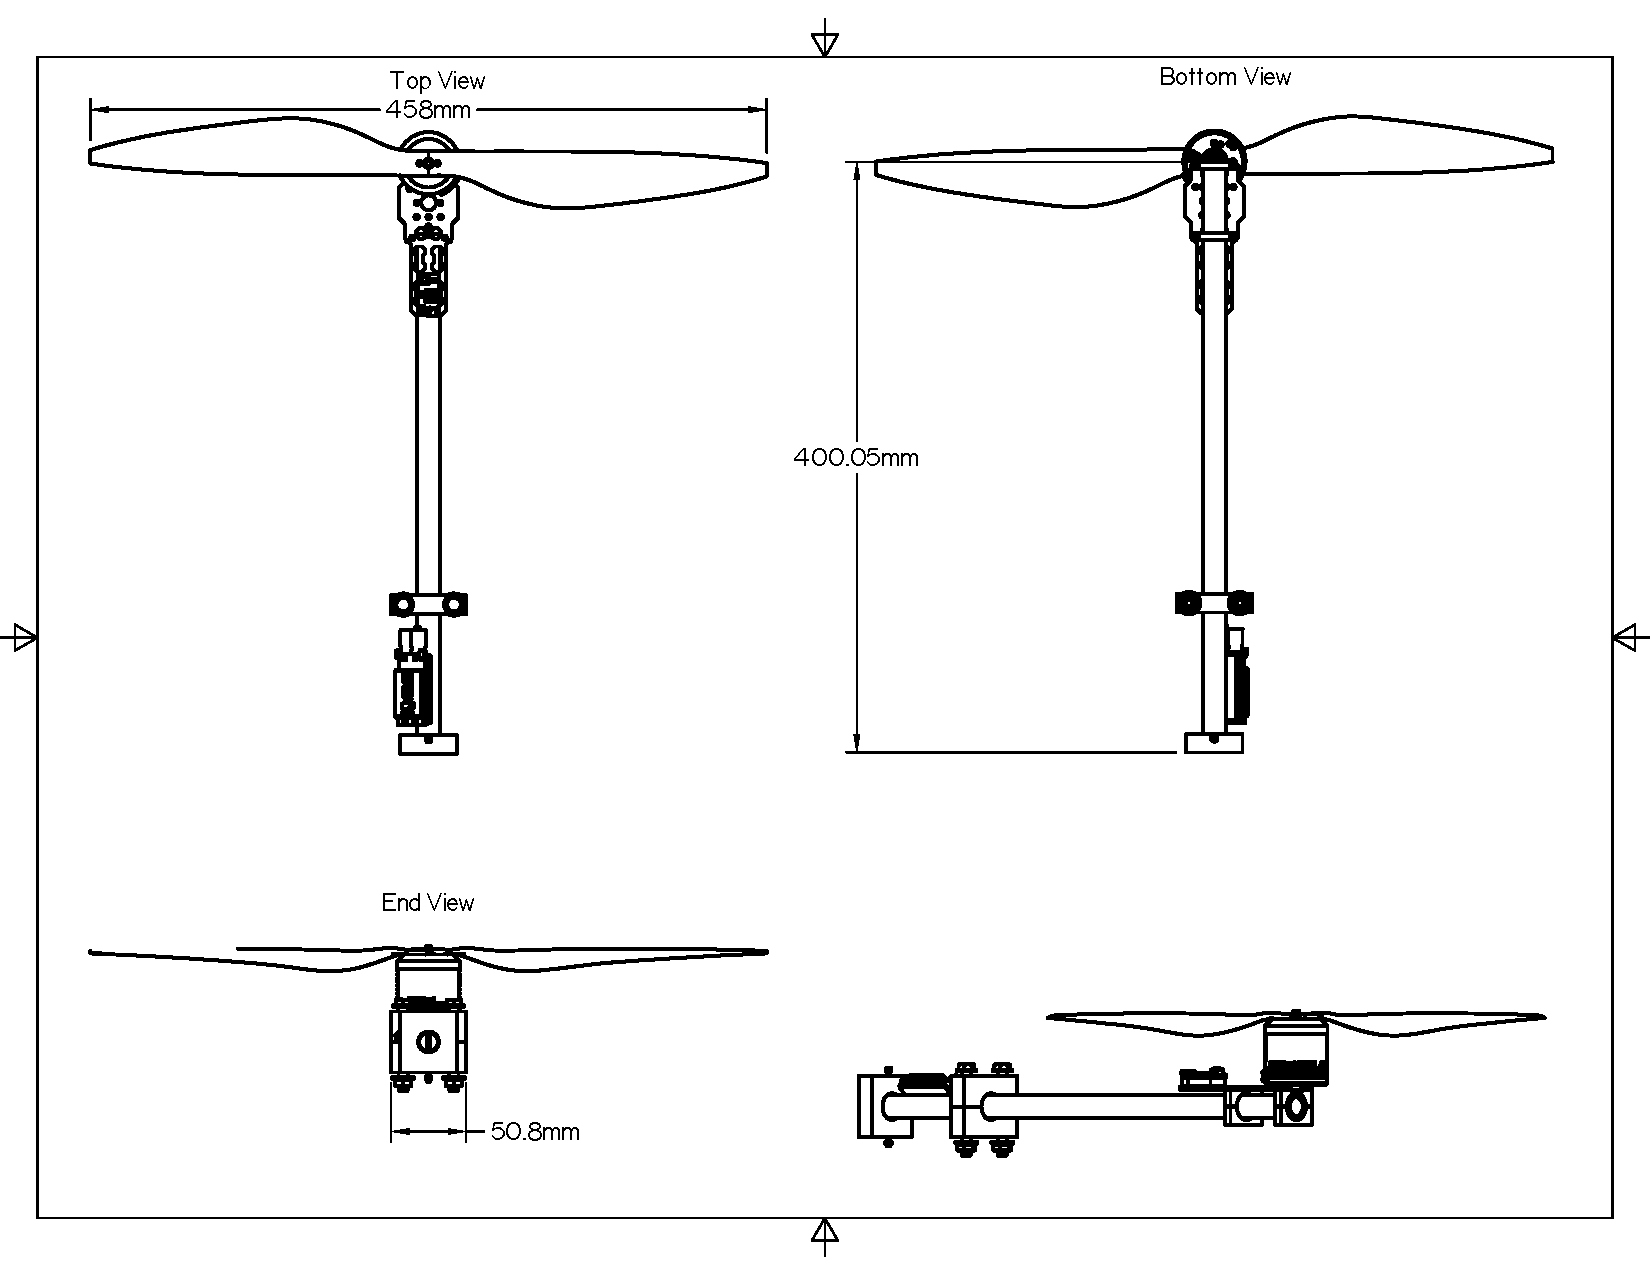
\includegraphics[width=1\linewidth]{system_diagrams/system_diagrams_Part7.pdf}
        \caption{Propeller Arm Dimensions}
        \label{fig:SystemDiagram7}
    \end{figure}

    \subsection{Airframe Performance}\label{ssec:airframeperformance}
        \subsubsection{Maximum Velocity} The maximum velocity safely tested on the MARS aircraft was 15 m/s in a straight line. Exceeding this velocity risks instability, especially in windy conditions.
        \subsubsection{Radio Connectivity Range} The MARS aircraft loses connection after flying approximately 1 km away from the \ac{gcs}. This was tested in a wooded environment with the \ac{gcs} on the ground and the done flying at an altitude of 60 meters relative to the \ac{gcs}. The antennas used were two 900 MHz 5 dBi omnidirectional rubber duck antennas. Higher range is expected with higher gain antennas and a higher \ac{gcs} with a direct line of sight to the aircraft.
        \subsubsection{Flight Duration} The maximum flight duration of the MARS aircraft is 17 minutes and 10 seconds at a hover. This test was conducted in a 36 degree Fahrenheit outdoor environment with a fully charged 23000 mAh battery and a 4.41 lbs payload. The starting battery voltage was 25.1V and the ending battery voltage was 20.83.

    \subsection{Radios}\label{ssec:c2systems}
        \subsubsection{Onboard Radio} The MARS aircraft is equipped with a Doodle Labs Mesh Rider Mini OEM radio (RM-1700-22M3). View the manufacturer's documentation \textcolor{blue}{\href{https://techlibrary.doodlelabs.com/mini-oem-dual-band-mesh-rider-radio-915-mhz-and-2450-mhz-ism-bands}{here}}.
        \begin{figure}[H]
            \centering
            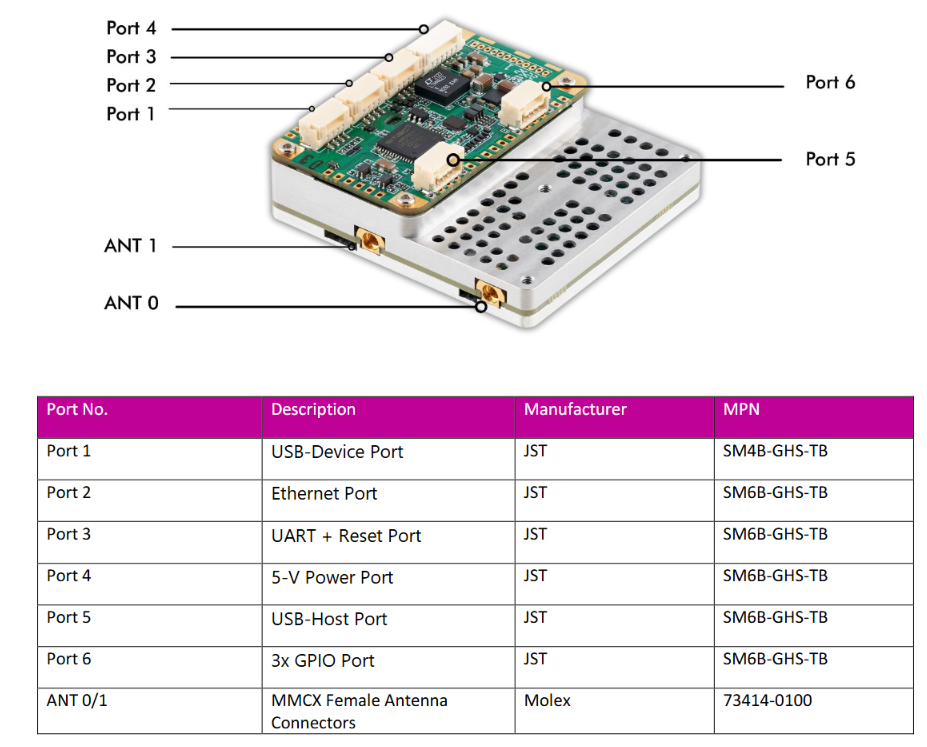
\includegraphics[width=0.5\linewidth]{Mini-OEM_port_diagram.png}
            \caption{Doodle Labs Mesh Rider Mini OEM Port Diagram}
            \label{fig:Mini_Ports}
        \end{figure}

        \begin{figure}[H]
            \centering
            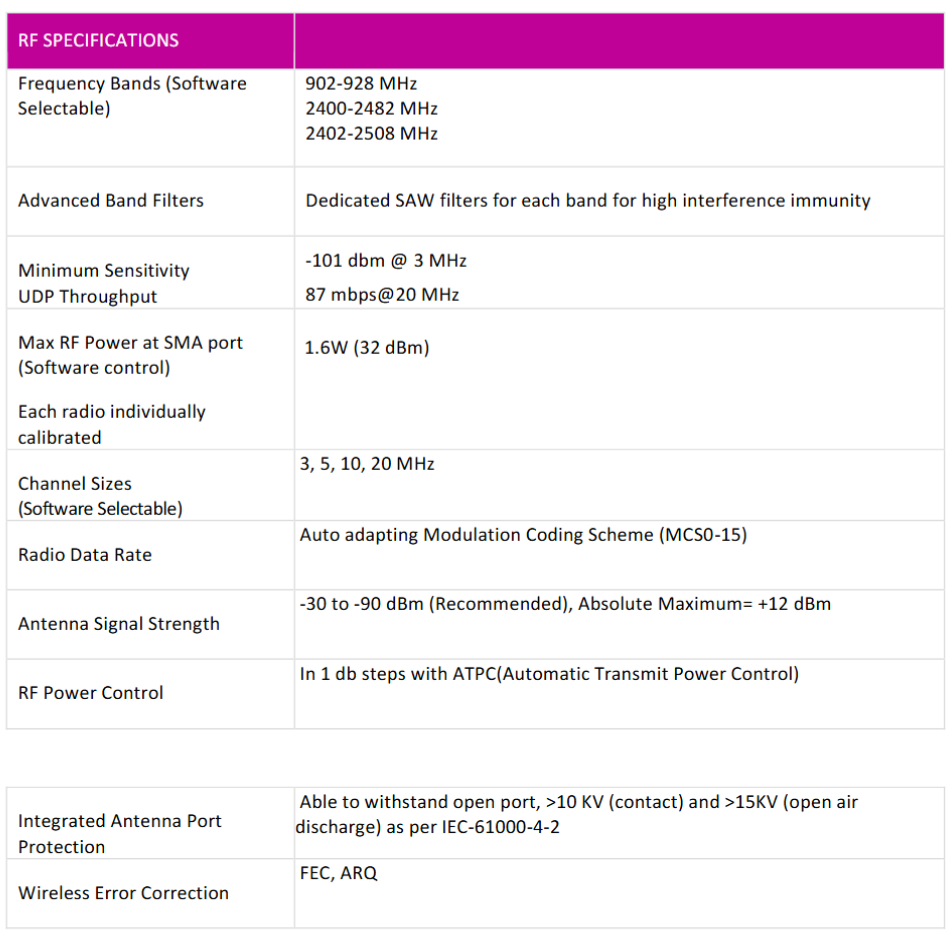
\includegraphics[width=0.5\linewidth]{Mini-OEM_RF_Specifications.png}
            \caption{Doodle Labs Mesh Rider Mini OEM RF Specifications}
            \label{fig:Mini_RF}
        \end{figure}
        \begin{figure}
            \centering
            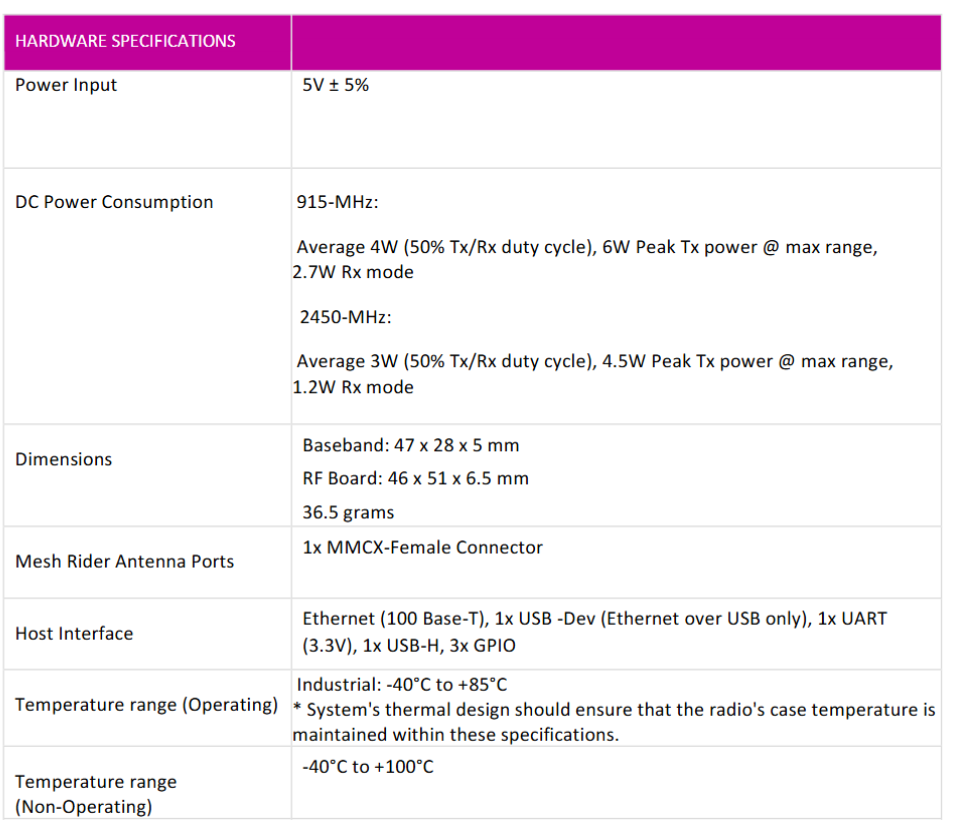
\includegraphics[width=0.5\linewidth]{Mini-OEM_HW_Specifications.png}
            \caption{Doodle Labs Mesh Rider Mini OEM Hardware Specifications}
            \label{fig:Mini_HW}
        \end{figure}

        \subsubsection{\ac{gcs} Radio}
        The radio used for the MARS GCS is the Doodle Labs Mesh Rider OEM (RM-1700-22O3). View the manufacturer's documentation \textcolor{blue} {\href{https://techlibrary.doodlelabs.com/multiband-oem-mesh-rider-radio-915-mhz-and-2450-mhz-ism-bands-1}{here}}.

        \begin{figure}[H]
            \centering
            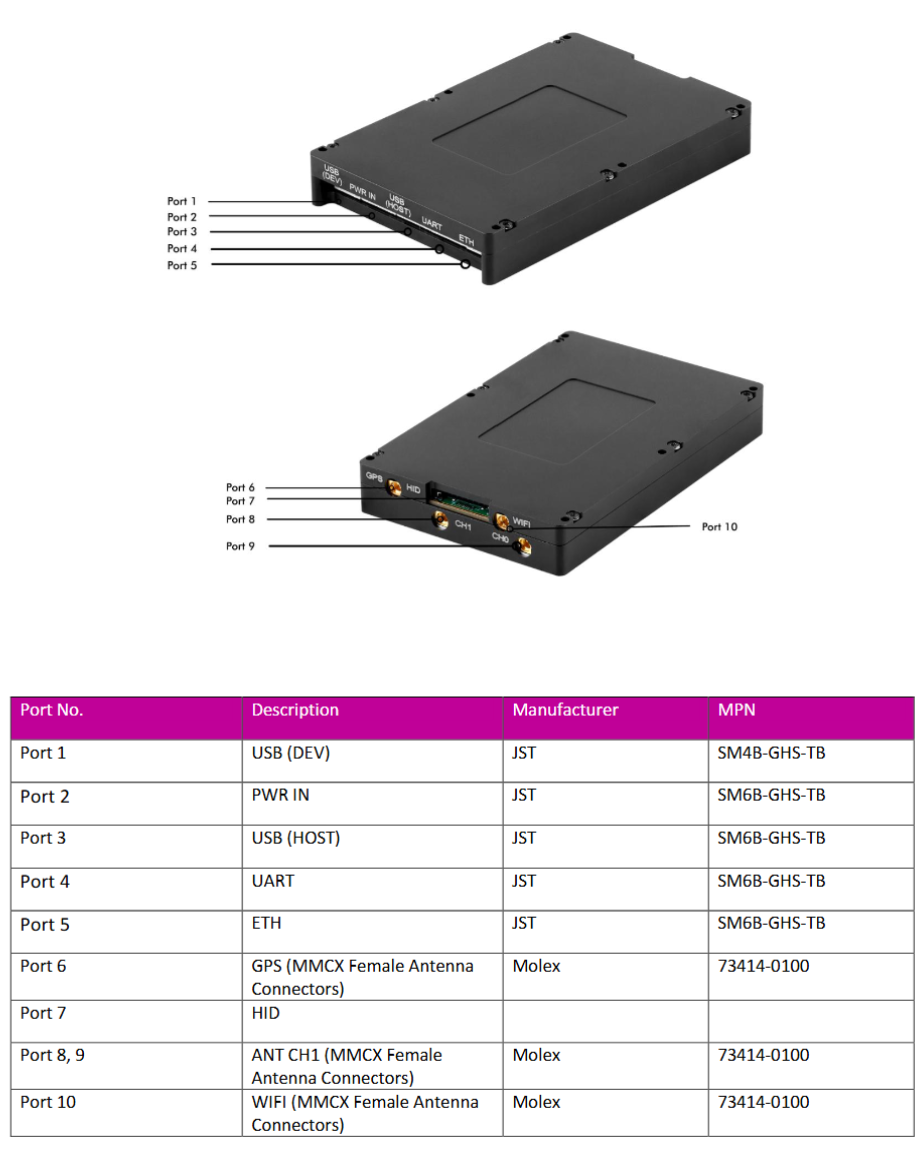
\includegraphics[width=0.5\linewidth]{OEM_Port_Diagram.png}
            \caption{Doodle Labs Mesh Rider OEM Port Diagram}
            \label{fig:OEM_Ports}
        \end{figure}

        \begin{figure}[H]
            \centering
            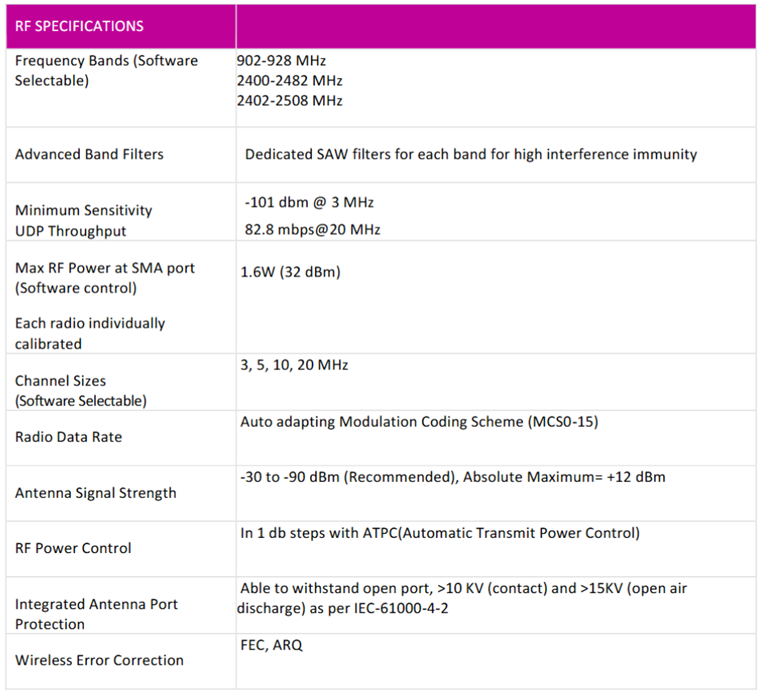
\includegraphics[width=0.5\linewidth]{OEM_RF_Specifications.png}
            \caption{Doodle Labs Mesh Rider OEM RF Specifications}
            \label{fig:OEM_RF}
        \end{figure}

        \begin{figure}[H]
            \centering
            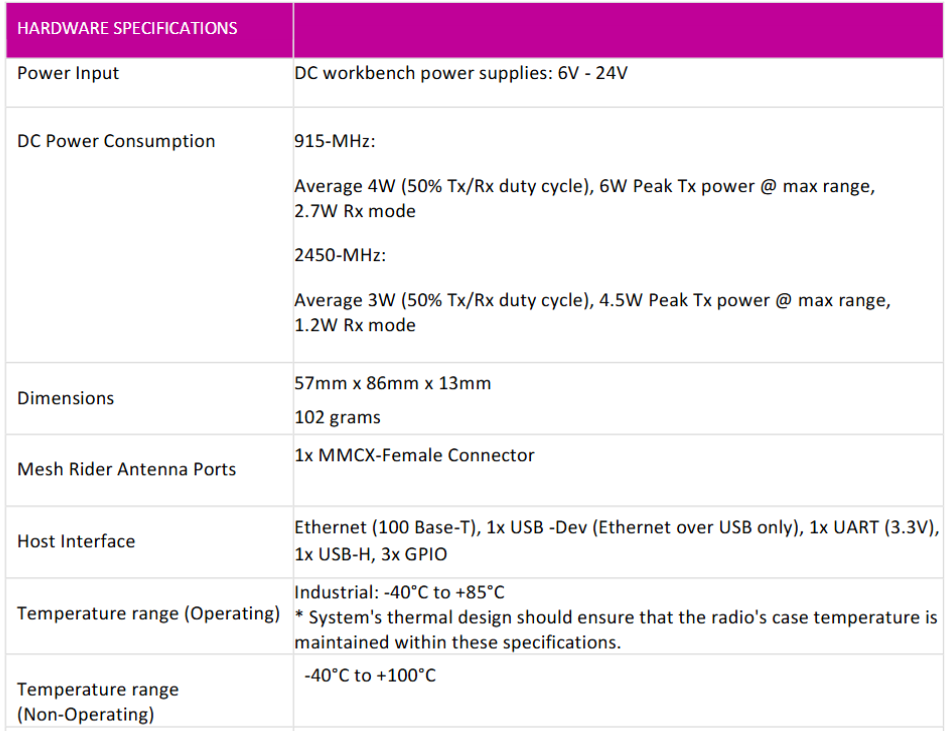
\includegraphics[width=0.5\linewidth]{OEM_HW_Specifications.png}
            \caption{Doodle Labs Mesh Rider OEM Hardware Specifications}
            \label{fig:OEM_HW}
        \end{figure}
    
    \subsection{\ac{bvlos} Systems}\label{ssec:bvlossystems}
    
\section{Cargo Approved for Flight}\label{sec:approvedcargo}
The MARS aircraft is rated to carry a payload of 5 lbs or lesss. The KACH Hospital Commander holds the authority for approving categories of cargo or for payloads heavier than 5 lbs. As of May 2026, the MARS aircraft is approved transporting the following MEDLOG items:
\begin{itemize}
    \item All over-the counter medication
    \item Prescription drugs
    \item Lab samples
    \item miscellaneous supplies such as bandages, gauze, latex gloves, isopropyl alcohol, etc.
\end{itemize}
As of May 2026, the MARS aircraft is not approved for any temperature-controlled substances or samples such as blood or insulin. However, the KACH Commander may implement temperature controls to enable transport of temperature-sensitive \ac{medlog}  at his/her own risk.

\section{\ac{gcs} and Software}\label{sec:gcssoftware}
\subsection{ArduPilot}
ArduPilot is an open-source software ecosystem designed for custom-built aircraft. It is comprised of the Mission Planner ground control software and the ArduPilot flight controller firmware. The Cube Orange+ flight controller onboard the MARS aircraft is installed with version 4.6.3 of the Ardupilot Copter firmware. This firmware is custom-configured with to include certain packages like RemoteID and Rangefinder. Visit https://custom.ardupilot.org/ to build a custom ArduPilot firmware for your flight controller.

\subsection{Ground Control Software}
MARS is compatible and tested with two open-source ground control softwares, Mission Planner, and QGroundControl. Both are compatible with the ArduPilot firmware, enabling them be used interchangeably at the preference of the operator.
    \subsubsection{Mission Planner}
    Mission Planner is the recommended ground control software due to its wide usage by the hobby drone community and its thorough documentation and tutorials available on Ardupilot.org and YouTube. Visit the Mission Planner page on Ardupilot.org: https://ardupilot.org/planner/
        
    \subsubsection{QGroundControl}
    QGroundControl is another option for ground control software. While it is designed for use with with PX4 flight controller firmware, it is still compatible with ArduPilot. However, this means that almost all tutorials and documentation for QGroundControl is specific to PX4 firmware, and it will not necessarily be applicable to a system running ArduPilot firmware. For this reason, it is recommended to use Mission Planner instead unless migrating over to PX4.

\subsection{Ground Control Station Hardware}
    \subsubsection{} The ground control station (GCS) consists of the following components:
    \begin{itemize}
        \item Doodle Labs Multiband OEM Mesh Rider Radio
        \item Human Interface Device (HID) board
        \item Evaluation board
        \item Two 900 MHz 5 dBi omnidirectional rubber duck antennas
    \end{itemize}

    \subsubsection{} The mesh radio operates within a dynamic networking topology, allowing nodes to relay data and maintain connectivity in beyond line-of-sight or degraded environments.

    \subsubsection{} The HID board provides real-time status indication and limited manual interaction for diagnostics and control. The evaluation board serves as the primary interface for radio configuration, power distribution, and communication (e.g., Ethernet connectivity).

\subsubsection{} The system antennas are optimized for 900 MHz operation and provide omnidirectional coverage to support robust communication links.

\subsection{Communication Performance Parameters}
\subsubsection{} Optimal communication performance is achieved under the following conditions:
\begin{itemize}
    \item Received Signal Strength Indicator (RSSI): approximately $-60$ to $-70$ dBm
    \item Noise floor: approximately $-95$ to $-100$ dBm
    \item Data rates: approximately 3 Mbps (transmit) and 12 Mbps (receive)
    \item Latency: 5--25 ms
\end{itemize}

\subsubsection{} Maintaining these parameters ensures stable, low-latency communication, which is critical for real-time command, control, and telemetry operations.


